\documentclass[journal]{IEEEtran}
% SENTINEL v2 manuscript. Every number in this paper must come from a script
% in the repository (results/ -> tables/figures); see README in this folder.
\usepackage{amsmath,amssymb,amsthm}
\usepackage{graphicx}
\usepackage{booktabs}
\usepackage{adjustbox}
\usepackage{cite}
\usepackage{algorithm}
\usepackage{algpseudocode}
\usepackage{xcolor}
\newcommand{\todo}[1]{\textcolor{red}{[TODO: #1]}}
% Screenshot placeholder until the file exists in figures/ (see docs/SCREENSHOTS.md)
\newcommand{\maybeimg}[2]{\IfFileExists{#2}{\includegraphics[width=#1]{#2}}{%
  \fbox{\parbox[c][3cm][c]{\dimexpr #1-2\fboxsep-2\fboxrule\relax}{\centering\footnotesize\textcolor{red}{screenshot pending:}\\\tiny\texttt{\detokenize{#2}}}}}}
\newtheorem{lemma}{Lemma}
\newtheorem{proposition}{Proposition}
\newtheorem{corollary}{Corollary}
\theoremstyle{definition}
\newtheorem{definition}{Definition}
\newtheorem{assumption}{Assumption}

\begin{document}
\title{Information-Triggered Delivery for Timely Victim Reporting\\ in Infrastructure-Free UAV Search and Rescue}
\author{Karthik~KS, Nicholas~Christo~T, and Balaji~Ganesh~Rajagopal}
\maketitle

\begin{abstract}
Small UAV swarms with onboard thermal detectors can search disaster areas without infrastructure, but
a victim found by a UAV helps only once the report reaches the responders, over radio links that are
obstructed, fading and broken by UAV failures. Keeping the swarm connected at all times makes every
report immediate but confines the search; searching freely leaves delivery to chance. We present
SENTINEL, a decentralised framework that lets UAVs search freely and triggers delivery from the
information each UAV has confirmed, fuses thermal detections from several viewpoints so that occluded
angles cannot veto a clear one, and, while a report is being delivered, constrains the UAVs on the
delivery path with an outage model and a local minimum spanning tree so that preserved links remain
reliable for every feasible step. We bound the probability that a confirmed detection is lost before
it is secured and show that nearest-neighbour distance constraints do not preserve connectivity. In
about 11\,000 simulated missions against seven baselines tuned with the same budget (connectivity
control, potential fields, communication-aware PSO, MAPPO and sweep search), with 30 seeds per
setting and paired tests, SENTINEL reports 23--30\,\% more victims within 60\,s than the best
baseline in urban rubble under six failure models, is significantly better than all baselines for
3--50 UAVs on a 400\,m area, and is never significantly worse; PX4 software-in-the-loop flights in
Gazebo agree with the fast simulator. Ablations attribute the gains to the delivery trigger and the
fusion rule, not to continuous connectivity. The onboard YOLO26n detector matches YOLOv8n in accuracy
on HIT-UAV with 31\,\% less compute.
\end{abstract}

\begin{IEEEkeywords}
UAV swarms, intermittent connectivity, search and rescue, edge AI, particle swarm optimization, delay-tolerant networking.
\end{IEEEkeywords}

\section{Introduction}\label{sec:intro}

After earthquakes, floods and large fires, cellular and backhaul infrastructure is often unavailable
precisely where responders need information. Small multirotor UAVs carrying thermal cameras can
search such areas quickly, and onboard detectors now run in a few milliseconds on embedded GPUs, so
victims can be detected without streaming video to a server \cite{hituav}. What remains hard is
getting each detection to the responders \emph{in time}. Without infrastructure, a report travels
only over the UAVs' own short-range radio links, which are obstructed by buildings, fade, and break
when UAVs fail.

Two families of methods address the communication side. Connectivity-maintenance controllers keep
the swarm's communication graph connected at all times, either through the algebraic connectivity
of the graph \cite{sabattini2013,zavlanos2008} or through edge potentials that never let a link
break \cite{ji2007}. Every detection then reaches the responder immediately, but the whole swarm is
tied to the responder's neighbourhood, which limits how far it can search. Intermittent-connectivity
and data-ferrying approaches let robots disconnect and meet according to a schedule
\cite{kantaros2017}, or plan ferry routes to sources whose positions are known in advance
\cite{cui2023ferry,bafarassat2026aoi}. In search and rescue neither assumption fits well: the information
sources, the victims, are \emph{discovered by the search itself}, at unknown places and times.

In an earlier version of this system we coupled a thermal detector with particle swarm
optimisation (PSO) and a distance penalty that kept UAVs within 50\,m of their nearest neighbour.
That design has three limitations, which also shaped this work. A fixed distance does not describe
a radio link behind rubble; keeping the nearest neighbour close does not keep the network connected
(Lemma~\ref{lem:nn}); and the evaluation used a 25\,m area that is far smaller than the radio range,
in which, as we show in Section~\ref{sec:eval:sitl}, every method stays connected and the methods
cannot be told apart.

This paper studies the \emph{discovery--delivery trade-off} directly. We measure the share of
victims whose report reaches the responder within a deadline, and we treat connectivity as a means
to that end rather than as an objective. Our contributions are:
\begin{itemize}
\item \textbf{Information-triggered delivery.} Each UAV searches without connectivity constraints and
switches to a delivery mode when a victim it confirmed has not reached the responder after a hold
time $T_h$ (Section~\ref{sec:method}). Rendezvous are triggered by information that the search
itself discovers, rather than by a schedule or by known source locations. $T_h$ exposes the
trade-off explicitly, and we bound the probability that a confirmed detection is lost to UAV
failures before it is secured (Proposition~\ref{prop:exposure}).
\item \textbf{Corroborative multi-view sensing.} Weak detections request a lateral second view from a
neighbour, and views from different directions are fused so that occluded viewpoints cannot veto a
clear one (Section~\ref{sec:fusion}). In dense swarms this fusion rule is the largest single
contributor to performance.
\item \textbf{A link-preservation safety layer with guarantees.} While a delivery is in progress,
the UAVs on the delivery path constrain their steps using a realistic outage model (path loss,
obstructions, shadowing, fading, interference) and a local minimum spanning tree. Preserved links
remain reliable for every feasible step (Proposition~\ref{prop:link}), and the delivering component
stays connected (Corollary~\ref{cor:conn}). We show why nearest-neighbour constraints do not
suffice (Lemma~\ref{lem:nn}).
\item \textbf{A reproducible evaluation.} We compare against seven baselines covering
communication-aware optimisation, algebraic-connectivity control, potential-based topology control,
multi-agent reinforcement learning and classical sweep search, all tuned with the same budget. The
evaluation spans 3--50 UAVs, four channel profiles, six failure models, moving obstacles and
detector uncertainty, uses 30 seeds per configuration with paired significance tests, and is
cross-checked against PX4 software-in-the-loop flight in Gazebo. Code, scenarios and results are
released.
\end{itemize}

Across the scenarios SENTINEL reports 23--30\,\% more victims within 60\,s than the best baseline in
urban rubble under all failure models, and it is significantly better than all baselines on the
400\,m area at every swarm size from 3 to 50; in the harshest channel it is ahead of or tied with the
best baseline. The ablation shows where this comes from: the delivery trigger and the fusion rule
account for the gains, whereas the link-preservation layer has no significant effect on performance
and fulfils its safety role, with $3.4\times10^{-5}$ link violations per preserved link-step. We
also report what does not work as well: keeping the swarm connected at all times lowers on-time
reporting to 0.03--0.13; in small, dense swarms a MAPPO policy trained to convergence comes close to
SENTINEL (differences not significant for $N=10$--20 on the 200\,m area); and the thermal detector,
trained on real imagery, transfers poorly to rendered Gazebo scenes.

Section~\ref{sec:related} positions this work against prior approaches,
Section~\ref{sec:model} defines the system model and problem, Section~\ref{sec:method} presents
SENTINEL, Section~\ref{sec:impl} describes the implementation, Section~\ref{sec:eval} reports the
evaluation and Section~\ref{sec:discussion} discusses limitations.

\section{Related Work}\label{sec:related}

\paragraph{Continuous connectivity maintenance}
A large body of work keeps a multi-robot communication graph connected at all times. Zavlanos and
Pappas control the robots so that the graph Laplacian keeps a positive second eigenvalue
\cite{zavlanos2008}; Sabattini et al.\ estimate the algebraic connectivity $\lambda_2$ in a
decentralised way and follow its gradient without requiring local links to persist
\cite{sabattini2013}; Ji and Egerstedt preserve edges through potentials that grow unbounded as a
link approaches its range, with hysteresis on edge creation \cite{ji2007}. Local topology-control
rules such as the local minimum spanning tree (LMST) \cite{li2003lmst} reduce the set of links that
must be kept. These methods prove that connectivity is maintained, but under a disk communication
model and at the price of tying every robot to the network at every instant. Our baselines B3 and B4
implement the second and third approach (B3 with the exact $\lambda_2$), and our measurements show
that in large areas this tie lowers the share of victims reported in time. SENTINEL applies such
constraints only for the duration of a delivery (Proposition~\ref{prop:link}) and replaces the disk model by a predicted outage
model that accounts for obstructions and fading.

\paragraph{Intermittent connectivity, data ferrying and information age}
Kantaros and Zavlanos let robots disconnect and enforce that they meet at the vertices of a mobility
graph infinitely often, with meeting schedules specified in temporal logic \cite{kantaros2017}.
UAV data-ferrying and delay-tolerant designs carry data physically between sources and a sink
\cite{cui2023ferry,chandran2024disaster}, and age-of-information (AoI) formulations optimise how fresh the
collected data are \cite{kaul2012aoi,amodu2023aoi,bafarassat2026aoi}. These approaches assume that the sources (sensors) are
known in advance or that meetings follow a predefined schedule. In search and rescue the sources
are the victims, discovered online by the search itself; SENTINEL's rendezvous are triggered by
that discovered information, and our deadline metric is AoI-like (time from confirmation to the
responder).

\paragraph{Communication-aware swarm search and learning}
PSO and its variants are widely used for multi-UAV coverage and search \cite{clerc2002,phung2020mpso};
distributed planners such as DAPSO run a local PSO on each UAV and exchange information over local
links, but assume that communication is available when needed \cite{yang2024dapso}.
Communication-aware variants add link-quality terms to the fitness; our baseline B2 represents this
family with the same outage model as SENTINEL applied as a soft penalty to all neighbours. Distributed Bayesian search reduces
traffic by flooding only positive detections but assumes a connected, lossless network
\cite{niu2026eventbayes}, and decentralised mountain-SAR search uses distance-limited links without a
responder sink \cite{zhu2026mountain}. Multi-agent reinforcement learning, with MAPPO as a strong
general baseline \cite{yu2022mappo}, has been applied to UAV coverage and communication-aware
coordination \cite{shi2025symmetry}; we include MAPPO with the same observations and objective as
baseline B5.

\paragraph{Onboard thermal perception}
Thermal datasets such as HIT-UAV \cite{hituav} enable lightweight detectors that run on the UAV, and
recent YOLO generations target edge deployment by removing non-maximum suppression and reducing
compute \cite{yolo26}. We use such a detector as an enabling component and evaluate it on real
thermal imagery; we do not claim it as a contribution.

\paragraph{Positioning}
Table~\ref{tab:related} summarises the comparison. To our knowledge, no prior work combines
online-discovered information sources, an explicit reporting deadline, a channel model with
obstructions and fading, failure-aware evaluation, and provable link preservation during delivery
(Proposition~\ref{prop:link}).

\begin{table*}[t]\centering
\caption{Comparison with the closest approaches (\checkmark: addressed; $\circ$: partially; --: not addressed).}
\label{tab:related}
\begin{adjustbox}{max width=\textwidth}\begin{tabular}{lcccccc}\toprule
Approach & Sources discovered & Delivery deadline & Obstruction/fading & UAV & Connectivity & Free search \\
 & online & / timeliness metric & channel model & failures & proof (Prop.~\ref{prop:link}) & (no permanent tie) \\\midrule
$\lambda_2$ control \cite{zavlanos2008,sabattini2013} & -- & -- & -- & $\circ$ & \checkmark & -- \\
Edge potentials \cite{ji2007} & -- & -- & -- & -- & \checkmark & -- \\
Intermittent connectivity \cite{kantaros2017} & -- & $\circ$ & -- & -- & \checkmark & \checkmark \\
Data ferrying / DTN \cite{cui2023ferry,chandran2024disaster} & -- & \checkmark & $\circ$ & -- & -- & \checkmark \\
AoI UAV data collection \cite{kaul2012aoi,bafarassat2026aoi,amodu2023aoi} & -- & \checkmark & $\circ$ & -- & $\circ$ & \checkmark \\
Distributed PSO search \cite{yang2024dapso,phung2020mpso} & \checkmark & -- & -- & -- & -- & \checkmark \\
Event-driven Bayesian search \cite{niu2026eventbayes} & \checkmark & -- & -- & -- & -- & \checkmark \\
MARL coordination \cite{yu2022mappo,shi2025symmetry} & $\circ$ & $\circ$ & $\circ$ & $\circ$ & -- & \checkmark \\
Earlier SENTINEL design (B1) & \checkmark & -- & -- & $\circ$ & -- & $\circ$ \\
\textbf{SENTINEL (this work)} & \checkmark & \checkmark & \checkmark & \checkmark & \checkmark$^{\dagger}$ & \checkmark \\
\bottomrule
\multicolumn{7}{l}{\footnotesize $^{\dagger}$ during delivery, for feasible steps (Proposition~\ref{prop:link}, Corollary~\ref{cor:conn}).}
\end{tabular}\end{adjustbox}
\end{table*}

\section{System Model and Problem Formulation}\label{sec:model}

\subsection{Network and Mobility}
A swarm $\mathcal{U}=\{1,\dots,N\}$ of multirotor UAVs flies at a common altitude $h$ over a
disaster area $\mathcal{A}\subset\mathbb{R}^2$ containing static obstacles. Obstacles taller than
$h$ form a no-fly set $\mathcal{O}\subset\mathcal{A}$ and obstruct radio links; low rubble only
occludes ground targets. A responder radio (node $0$) is fixed at the launch point
$x_0\in\mathcal{A}$; it is the only sink for victim reports and is assumed not to fail. UAV $i$
has position $x_i(t)\in\mathcal{A}\setminus\mathcal{O}$ and speed $\|\dot x_i\|\le v$. Time is
slotted with control period $\Delta t$; every UAV broadcasts one beacon per slot containing its
position, its target ledger and acknowledgements (Section~\ref{sec:method}).

\subsection{Channel Model}
The received SINR of the broadcast from $i$ at $j$ in slot $t$ is
\begin{equation}
\gamma_{ij}(t)=\frac{P_t G^2\, 10^{-(\mathrm{PL}(d_{ij})+n_{ij}L_o+X_{ij})/10}\; |h_{ij}|^2}
{\sigma^2+\sum_{k\in\mathcal{I}_j(t)}\bar P_{kj}},\label{eq:sinr}
\end{equation}
where $\mathrm{PL}(d)=\mathrm{PL}(d_0)+10\eta\log_{10}(d/d_0)$ is log-distance path loss,
$n_{ij}$ the number of obstacles crossing the segment $[x_i,x_j]$ with per-obstruction loss $L_o$,
$X_{ij}\sim\mathcal{N}(0,\sigma_X^2)$ log-normal shadowing evolving with the Gudmundson
correlation $\rho=e^{-\Delta/d_c}$ for endpoint displacement $\Delta$, $|h_{ij}|^2$ unit-mean
Rician fading with factor $K$ ($K=0$, Rayleigh, once obstructed), and $\mathcal{I}_j(t)$ the set
of transmitters colliding in the slot, each present with probability $p_a$. A packet is decoded
iff $\gamma_{ij}\ge\gamma_{\mathrm{th}}$. The link outage probability, averaged over fading and
shadowing, is
\begin{equation}
P_{\mathrm{out}}(d,n)=\mathbb{E}_X\!\left[F_{|h|^2}\!\left(\frac{\gamma_{\mathrm{th}}}{\bar\gamma(d,n)\,10^{X/10}}\right)\right],
\label{eq:pout}
\end{equation}
with $F_{|h|^2}$ the non-central $\chi^2_2$ CDF (computed in closed form; the outer expectation
by Gauss--Hermite quadrature). The \emph{reliable range} for target outage $\varepsilon$ is
$R_\varepsilon(n)=\max\{d: P_{\mathrm{out}}(d,n)\le\varepsilon\}$, and the \emph{reliable graph}
$\mathcal{G}_\varepsilon(t)$ joins $i,j$ iff $P_{\mathrm{out}}(d_{ij},n_{ij})\le\varepsilon$.
Table~\ref{tab:channel} lists the four environment profiles; their parameters follow the ranges
reported for low-altitude aerial and street-level links \cite{tr36777,itup1411}, with
shadowing correlation following \cite{gudmundson1991}; they are not calibrated against measurements
in rubble (Section~\ref{sec:discussion}). For the urban-rubble profile $R_{0.05}(0)=91$\,m and $R_{0.05}(1)=48$\,m,
which places the fixed 50\,m range of the earlier SENTINEL design in context: it is the
reliable range of a link behind one obstruction, not a property of the radio alone.

\begin{table}[t]\centering\caption{Channel profiles ($f=2.4$\,GHz, $P_t=20$\,dBm, $B=20$\,MHz,
$\gamma_{\mathrm{th}}=5$\,dB) and resulting reliable ranges at $\varepsilon=0.05$.}\label{tab:channel}
\begin{tabular}{lcccccc}\toprule
Profile & $\eta$ & $\sigma_X$ & $K$ (LoS) & $L_o$ & $R(0)$ & $R(1)$\\\midrule
open & 2.0 & 2 & 10\,dB & 6\,dB & 2434\,m & 684\,m\\
suburban & 2.5 & 4 & 6\,dB & 10\,dB & 339\,m & 95\,m\\
urban-rubble & 3.0 & 6 & 3\,dB & 6\,dB & 91\,m & 48\,m\\
severe & 3.5 & 8 & Rayleigh & 8\,dB & 35\,m & 21\,m\\\bottomrule
\end{tabular}\end{table}

\subsection{Sensing Model}
Each UAV carries a nadir thermal camera with ground footprint radius $r_f$ and an onboard
detector (Section~\ref{sec:impl}). A look at a cell updates the residual probability that an
undetected victim is present by Bayes' rule, $p\leftarrow p(1-P_d)/(1-pP_d)$ \cite{stone1975}. The detector returns a confidence $c\in[0,1]$ whose distribution depends on
slant range and on view-dependent occlusion (calibrated from the detector, Section~\ref{sec:eval});
false positives from warm debris arrive as a Poisson process per look.

\subsection{Information Model}
Every UAV keeps a ledger of world-frame target entries. Observations within a gate are
associated to one entry; the best confidence per viewing sector is kept and the sectors are fused
into one confidence $c_e$ (Section~\ref{sec:fusion}). An entry is \emph{confirmed} when
$c_e\ge c_{\mathrm{hi}}$ and \emph{tentative} when $c_{\mathrm{lo}}\le c_e<c_{\mathrm{hi}}$.
Ledgers are replicated by gossip with acknowledgements, so each entry carries its holder set
$H_e(t)$. An entry is \emph{secured} once $0\in H_e$ (the responder holds it) and \emph{lost}
if it was confirmed but no alive node holds it.

\subsection{Failure Model}
UAVs fail by crashing (the node and its ledger copy disappear), by radio loss (it flies but
cannot communicate) or by gradual brownout (transmit power decays). We study single,
simultaneous, cascading and Poisson failures with per-UAV rate $\lambda_f$.

\subsection{Problem}
Let $\tau_k$ be the time victim $k$ is first confirmed by any UAV and $T_k\ge\tau_k$ the time
its report reaches the responder ($T_k=\infty$ if never). With mission horizon $T$ and value
discount $\theta$, the team maximises the time-discounted report value
\begin{equation}
J=\frac{1}{|\mathcal{V}|}\sum_{k\in\mathcal{V}} e^{-T_k/\theta},\label{eq:J}
\end{equation}
subject to the dynamics, $x_i\notin\mathcal{O}$, and decentralised information (each UAV acts on
its own sensing and on beacons it actually received). $J$ couples three quantities that prior
work optimises separately: discovery (a victim must be found), delivery (its report must reach
the responder), and timeliness (sooner is better, in the spirit of age of information
\cite{kaul2012aoi}). Maintaining $\mathcal{G}_\varepsilon$ connected at all times makes delivery
immediate but restricts discovery; pure exploration maximises discovery but leaves delivery to
chance contacts, so confirmed information can wait arbitrarily long or be lost with its carrier.
We refer to this tension as the \emph{discovery--delivery trade-off}.

\section{SENTINEL}\label{sec:method}

Each UAV runs the same decentralised agent (Algorithm~\ref{alg:agent}), built from three parts.
(i)~\emph{Information-triggered delivery}: the agent alternates between two modes driven by its own
information state; in \textsc{Explore} it searches without any connectivity constraint, in
\textsc{Deliver} it returns toward the responder until the victims it has confirmed are secured.
(ii)~\emph{Corroborative multi-view sensing}: weak detections request a second viewpoint from a
neighbour, and views are fused so that occluded angles cannot veto a clear one.
(iii)~\emph{A link-preservation safety layer}: while delivering, a UAV and the relays between it and
the responder constrain their motion so that the links they rely on stay reliable, with a
guarantee for feasible steps (Proposition~\ref{prop:link}). Section~\ref{sec:eval:ablation} shows that (i) and (ii) produce the
performance gains, while (iii) ensures that deliveries are not interrupted by the swarm's own
motion.

\subsection{Mode switching}
Let $\mathcal{E}_i(t)$ be the confirmed entries held by UAV $i$ that are not secured and for which
$i$ is responsible (it created them, or the creator has been silent for $3T_h$, i.e.\ the copy is
orphaned). UAV $i$ switches to \textsc{Deliver} when the oldest such entry reaches age $T_h$,
\begin{equation}
\max_{e\in\mathcal{E}_i(t)}\,(t-\tau_e)\;\ge\;T_h,\label{eq:trigger}
\end{equation}
and back to \textsc{Explore} when $\mathcal{E}_i(t)=\emptyset$. The hold time $T_h$ is the single
parameter that trades discovery against delivery latency: $T_h=0$ delivers every confirmation
immediately, $T_h\to\infty$ never interrupts the search. Whether a UAV is connected to the
responder is known locally from a heartbeat: the responder stamps its beacons with the current
time and every UAV relays the freshest stamp it received; UAV $i$ is \emph{connected} if its
freshest stamp is younger than $T_{\mathrm{hb}}$.

\subsection{Waypoint optimisation (EM-PSO)}
Every planning period the agent chooses its next waypoint inside the reachable disk
$\mathcal{D}_i=\{x:\|x-x_i\|\le v T_p\}\setminus\mathcal{O}$ by maximising
\begin{multline}
F_i(x)=w_c\,\hat G_i(x)+w_d\!\!\sum_{e\in\mathcal{T}_i}\!c_e\,e^{-\frac{\|x-x_e\|^2}{2s^2}}\\
+w_g\,\frac{\|x_i-g_i\|-\|x-g_i\|}{vT_p}-S_i(x),\label{eq:fitness}
\end{multline}
where $\hat G_i(x)$ is the normalised expected number of detections of a look at $x$ computed on
the UAV's own search map (cells inside footprints claimed by neighbours removed), $\mathcal{T}_i$
the tentative entries, and $g_i$ a frontier goal (the map cell maximising expected detections
discounted by distance). The \emph{signal spring} acts only while the UAV is tethered (in
\textsc{Deliver} and connected, or holding a relay tether, Section~\ref{sec:tether}):
\begin{equation}
S_i(x)=\lambda_i\sum_{j\in\mathcal{S}_i}\left(\frac{[P_{\mathrm{out}}(\|x-x_j\|,n(x,x_j))-\varepsilon_i]_+}{\varepsilon_i}\right)^2,
\label{eq:spring}
\end{equation}
with $\lambda_i=\lambda_0(1+\beta U_i)$ and $\varepsilon_i=\varepsilon/(1+\beta U_i)$, where $U_i$ is the
number of entries only $i$ holds. Unlike a distance penalty, \eqref{eq:spring} penalises the
predicted \emph{outage} of the link, so it accounts for obstructions and fading, and it tightens
with the amount of unique information the UAV carries. The maximisation uses a
constriction-coefficient PSO ($\chi=0.7298$, $c_1=c_2=2.05$) \cite{clerc2002}, whose
particles are seeded with the previous waypoint, the step toward $g_i$ and the waypoints
broadcast by neighbours.

\subsection{Link preservation (safety layer)}\label{sec:proj}
The spring~\eqref{eq:spring} steers the search toward reliable links but cannot ensure that they
survive. While tethered, UAV $i$ therefore projects its step onto a feasible set built from its
preserved neighbours $\mathcal{S}_i$.

\begin{definition}[Local MST neighbours]
Let $\hat{\mathcal{G}}_i$ be the subgraph of the reliable graph induced by $i$ and the neighbours it
heard within the last $T_{\mathrm{hb}}$, with edge weights $(d_{jk},\max(j,k),\min(j,k))$ ordered
lexicographically. $\mathcal{S}_i$ is the set of neighbours adjacent to $i$ in the minimum
spanning tree of $\hat{\mathcal{G}}_i$ \cite{li2003lmst}.
\end{definition}

\begin{lemma}[Nearest-neighbour constraints do not imply connectivity]\label{lem:nn}
There are configurations in which every UAV is within $R$ of its nearest neighbour while the
communication graph is disconnected.
\end{lemma}
\begin{proof}
Four UAVs at $(0,0),(10,0),(200,0),(210,0)$ with $R=50$\,m: each has a neighbour at 10\,m, yet no
edge joins $\{1,2\}$ to $\{3,4\}$.
\end{proof}
Lemma~\ref{lem:nn} is why the nearest-neighbour spring of the earlier SENTINEL design cannot certify
network maintenance.

\begin{lemma}[LMST spans the reliable graph \cite{li2003lmst}]\label{lem:lmst}
Let $\mathcal{G}^-$ contain edge $(i,j)$ iff $j\in\mathcal{S}_i$ and $i\in\mathcal{S}_j$, all
computed from the same positions. Then $\mathcal{G}^-$ contains the minimum spanning forest of
the reliable graph, hence has the same connected components.
\end{lemma}
\begin{proof}
Let $(i,j)$ be an edge of the global minimum spanning forest $\mathcal{M}$. If $(i,j)$ were not
in the local MST of $\hat{\mathcal{G}}_i$, the cycle property would give a cycle in
$\hat{\mathcal{G}}_i$ on which $(i,j)$ is the unique heaviest edge; that cycle exists in the
reliable graph, contradicting $(i,j)\in\mathcal{M}$. The same holds for $\hat{\mathcal{G}}_j$, so
$(i,j)\in\mathcal{G}^-$. Since $\mathcal{M}\subseteq\mathcal{G}^-$ and $\mathcal{G}^-$ only uses
reliable links, the components coincide.
\end{proof}

\paragraph{Midpoint-ball projection}
For each $j\in\mathcal{S}_i$ let $\hat x_j$ be $j$'s last reported position, of age $a_{ij}$,
$m_{ij}=(x_i+\hat x_j)/2$, and $\delta_{ij}=v(\Delta t+a_{ij})$ the furthest $j$ can move before
the next check. The proposed step $u_i$ is scaled to the largest $\alpha\in[0,1]$ such that
$x_i'=x_i+\alpha u_i$ satisfies, for all $j\in\mathcal{S}_i$,
\begin{equation}
\|x_i'-m_{ij}\|\le \tfrac12 r_{ij}(x_i')-\tfrac12 v\,a_{ij},\quad
r_{ij}(x_i')=R_\varepsilon\big(n^{\delta_{ij}}(x_i',\hat x_j)\big),\label{eq:proj}
\end{equation}
where $n^{\delta}(a,b)$ counts obstacles inflated by $\delta$ that cross $[a,b]$. If no
$\alpha>0$ satisfies \eqref{eq:proj} the UAV hovers, or, if it is already outside a constraint,
takes the largest step toward the violated centre that does not enlarge any other violation.
Each UAV evaluates \eqref{eq:proj} with local information only.

\begin{proposition}[Link preservation]\label{prop:link}
Suppose $j\in\mathcal{S}_i$ and $i\in\mathcal{S}_j$, both UAVs are tethered, speeds are
bounded by $v$, positions are exchanged with staleness at most $a$, and the steps of both
UAVs satisfy \eqref{eq:proj}. Then the link $(i,j)$ is $\varepsilon$-reliable at $t+\Delta t$.
\end{proposition}
\begin{proof}
Let $m=(x_i+x_j)/2$ be the true midpoint. Since $\|\hat x_j-x_j\|\le va_{ij}$, we have
$\|m_{ij}-m\|\le va_{ij}/2$ and, symmetrically, $\|m_{ji}-m\|\le va_{ji}/2$. By \eqref{eq:proj} and
the triangle inequality,
$\|x_i'-x_j'\|\le\|x_i'-m_{ij}\|+\|m_{ij}-m\|+\|m-m_{ji}\|+\|m_{ji}-x_j'\|\le\tfrac12(r_{ij}+r_{ji})$.
The segment $[x_i',x_j']$ lies within $\|x_j'-\hat x_j\|\le\delta_{ij}$ of $[x_i',\hat x_j]$, so
every obstacle crossing it, un-inflated, crosses $[x_i',\hat x_j]$ when inflated by
$\delta_{ij}$: $n(x_i',x_j')\le n^{\delta_{ij}}(x_i',\hat x_j)$ and, $R_\varepsilon$ being
non-increasing in $n$, $R_\varepsilon(n(x_i',x_j'))\ge r_{ij}$. Likewise
$R_\varepsilon(n(x_i',x_j'))\ge r_{ji}$. Hence
$\|x_i'-x_j'\|\le\max(r_{ij},r_{ji})\le R_\varepsilon(n(x_i',x_j'))$.
\end{proof}

\begin{corollary}[Connectivity during delivery]\label{cor:conn}
If all UAVs of a connected component of $\mathcal{G}_\varepsilon(t)$ containing the responder
are tethered, take steps satisfying \eqref{eq:proj}, and no UAV fails, that component remains
connected at $t+\Delta t$.
\end{corollary}
\noindent\emph{Remark.} Proposition~\ref{prop:link} is a one-step guarantee for feasible steps;
it does not by itself make \eqref{eq:proj} feasible at every step (the inflated obstruction count
can shrink $r_{ij}$ even for a hovering UAV). We therefore also report the empirical rate of
preserved-link violations in all experiments, and a Monte-Carlo check of the obstacle-free
synchronous case ($10^4$ random swarms of 2--50 UAVs, 25 adversarial steps each, no violation).
\begin{proof}
By Lemma~\ref{lem:lmst} the mutually selected edges span the component, and by
Proposition~\ref{prop:link} each of them is reliable at $t+\Delta t$ (the responder never moves,
so a one-sided constraint suffices for its edges).
\end{proof}

\begin{proposition}[Probabilistic delivery path]\label{prop:prob}
Under Corollary~\ref{cor:conn}, the probability that, in a slot, the realised (fading) network
restricted to the preserved spanning tree $\mathcal{M}$ is disconnected satisfies
$\Pr[\text{disc.}]\le\sum_{e\in\mathcal{M}}P_{\mathrm{out}}(e)\le(|\mathcal{M}|)\,\varepsilon$.
\end{proposition}
\begin{proof}
The realised tree is disconnected only if at least one of its edges is in outage; apply the union
bound and $P_{\mathrm{out}}(e)\le\varepsilon$ for preserved edges.
\end{proof}

\subsection{Relay tether}\label{sec:tether}
Proposition~\ref{prop:link} needs \emph{both} endpoints tethered, but the relays between a
delivering UAV and the responder are usually exploring. A delivering, connected UAV therefore
stamps $t_{\mathrm{tether}}=t+T_{\mathrm{rel}}$ in its beacon; stamps propagate by maximum, and a
connected UAV is tethered while $t\le t_{\mathrm{tether}}$. The whole connected component thus
holds its links during a delivery and is released $T_{\mathrm{rel}}$ after it ends; because the
stamp is set only by delivering UAVs, tethers cannot sustain each other indefinitely.

\subsection{Information exposure}
\begin{proposition}[Exposure bound]\label{prop:exposure}
Assume the creator of a confirmed entry stays alive until it is secured or fails, flies at speed
$v$ along paths at most $\kappa\ge1$ times the straight-line distance, and that delivery
completes within $\tau_c$ of reaching the responder's connected component. Then the entry is
unsecured for at most $W=T_h+\kappa D/v+\tau_c$, with $D=\max_{x\in\mathcal{A}}\|x-x_0\|$. If the
UAVs holding it fail independently at rate $\lambda_f$ and the entry has $k$ holders during
that window,
\begin{equation}
\Pr[\text{entry lost}]\le\left(1-e^{-\lambda_f W}\right)^k\le(\lambda_f W)^k.\label{eq:exposure}
\end{equation}
\end{proposition}
\begin{proof}
By \eqref{eq:trigger}, \textsc{Deliver} starts at most $T_h$ after confirmation; the return takes
at most $\kappa D/v$ and the hand-off at most $\tau_c$, after which $0\in H_e$ and the entry is
secured (the responder does not fail). It is lost only if every holder fails within the window,
which has probability $(1-e^{-\lambda_fW})^k$ under independence; $1-e^{-z}\le z$.
\end{proof}
Proposition~\ref{prop:exposure} makes the role of $T_h$ explicit: it bounds the exposure of
confirmed information to UAV failures (the information-loss side), while larger $T_h$ leaves
more time for search (the discovery side). Section~\ref{sec:eval} measures the resulting
trade-off and compares the measured losses with \eqref{eq:exposure}.

\subsection{Collaborative synthetic-aperture sensing}
A tentative entry ($c_{\mathrm{lo}}\le c_e<c_{\mathrm{hi}}$) requests a second view from the
nearest neighbour at a lateral offset of $\pm b$ ($b=15$\,m) perpendicular to the observer--target
direction, admitted only if the flank point keeps that neighbour's preserved links feasible.
The flanking view enters the corroborative fusion below.

\subsection{Corroborative multi-view fusion}\label{sec:fusion}
A victim is observed by several UAVs from different directions. For each entry the ledger keeps the
best confidence $c_{e,v}$ per viewing sector $v$ (eight azimuth sectors around the entry), so repeated
frames from one viewpoint are not counted twice. The textbook naive-Bayes rule
$\mathrm{logit}\,c_e=\sum_v\mathrm{logit}\,c_{e,v}$ treats every low-confidence view as evidence
\emph{against} a victim. Under occlusion this is wrong: a victim partly covered by a slab returns weak
detections from the occluded side and strong ones from the open side, and a weak view from a blocked
angle says little about absence. With many UAVs the many weak views outvote a clear view and the
victim is never confirmed. We therefore fuse corroboratively,
\begin{equation}
\mathrm{logit}\,c_e=\max_v\mathrm{logit}\,c_{e,v}+\sum_{v\neq v^\star}\big[\mathrm{logit}\,c_{e,v}\big]_+,
\label{eq:fusion}
\end{equation}
where $v^\star$ is the best view: the best view sets the confidence, other views can only add
corroborating evidence, and a single view keeps its own confidence. Equation~\eqref{eq:fusion} is
the component with the largest measured effect in dense swarms (Section~\ref{sec:eval:ablation}); its
cost is that two independent false alarms on the same spot corroborate each other, which we evaluate
with deliberately adverse clutter (Section~\ref{sec:eval:uncertainty}).

\subsection{Complexity}
Per planning step a UAV evaluates $P$ particles for $I$ iterations; each evaluation costs
$O(k)$ for $k=|\mathcal{S}_i|$ outage look-ups plus an $O(1)$ map look-up (the footprint
convolution is computed once per step, $O(M)$ for $M$ map cells). The local MST costs
$O(k_h^2\log k_h)$ for the $k_h$ neighbours heard. None of these terms depends on $N$; the
measured per-agent compute time versus $N$ is reported in Section~\ref{sec:eval}.

\begin{algorithm}[t]\caption{SENTINEL agent $i$ (every slot $\Delta t$)}\label{alg:agent}
\begin{algorithmic}[1]
\State sense: record look, add geolocated detections to the ledger (fused per viewpoint)
\State broadcast beacon $(x_i,\text{ledger},\text{acks},\text{heartbeat},t_{\mathrm{tether}})$; merge received beacons
\If{planning slot}
  \State update mode with \eqref{eq:trigger}; issue SA flank requests for own tentative entries
  \If{\textsc{Deliver} and not connected} \State waypoint $\gets x_0$
  \Else \State waypoint $\gets\arg\max_{x\in\mathcal{D}_i}F_i(x)$ by PSO \Comment{$S_i\equiv0$ unless tethered}
  \EndIf
\EndIf
\State $u_i\gets$ step toward waypoint (rotated away from $\mathcal{O}$)
\If{tethered} \State $u_i\gets\alpha^\star u_i$ with $\alpha^\star$ from \eqref{eq:proj} \EndIf
\State fly $x_i\gets x_i+u_i$
\end{algorithmic}
\end{algorithm}

\section{Implementation}\label{sec:impl}

\paragraph{One algorithm library, two execution environments}
All algorithms of Section~\ref{sec:method} (channel model, ledger, fusion, PSO, link preservation,
delivery trigger) are implemented once in a ROS-independent Python library. The same library is
executed by (i) a fast multi-agent simulator used for the statistical evaluation and (ii) ROS~2
Humble nodes that fly PX4 multicopters in Gazebo Harmonic, so the results of both environments
refer to identical decision code.

\paragraph{Flight stack}
Each UAV is a PX4 x500 quadrotor with a nadir thermal camera (640$\times$512, 50$^\circ$ field of
view, 10\,Hz, radiometric 16-bit output converted to white-hot 8-bit on board). PX4 runs as
software-in-the-loop; the Micro XRCE-DDS agent bridges its uORB topics to ROS~2. Per UAV, four nodes
run on the companion computer (Fig.~\ref{fig:graph}): \texttt{flight\_commander} (offboard position
control and world-frame pose), \texttt{thermal\_vision} (YOLO26n detection and geolocation of every
box into the world frame from the camera model, pose and heading), \texttt{emps\_agent} (the
SENTINEL agent) and the camera bridge. There is no central coordinator.

\paragraph{Radio emulation and failures}
All inter-UAV beacons pass through a \texttt{comm\_emulator} node that delivers each packet only if
its sampled SINR, computed with the channel model of Section~\ref{sec:model} and the building
geometry of the world, exceeds the decoding threshold; it also hosts the responder radio. A
\texttt{chaos\_monkey} node injects crashes (force-disarm), radio cuts and brownouts on a schedule,
and a \texttt{metrics\_logger} computes the metrics of Section~\ref{sec:eval} from ground truth. A
beacon carries the sender's position, ledger, acknowledgements and heartbeat; it averages 4.1\,kB
(20\,kB when the search map is included every fourth beacon).

\paragraph{Disaster scenes}
Worlds are generated procedurally from a seed: tall building shells (no-fly, link-obstructing), low
rubble that occludes victims, warm debris (316\,K) that causes false alarms, and Rescue Randy
mannequins with a 310\,K body heat signature, partly or fully covered by concrete slabs
(Figs.~\ref{fig:world}--\ref{fig:occlusion}). The same seed produces the same scene in Gazebo and in
the fast simulator, which is what makes the cross-check of Section~\ref{sec:eval:sitl} possible.

\begin{figure}[t]\centering
\maybeimg{\columnwidth}{figures/S1_world_overview.png}
\caption{Generated 100\,m disaster area in Gazebo Harmonic (top view): building shells, rubble,
warm debris and victims.}\label{fig:world}
\end{figure}
\begin{figure}[t]\centering
\maybeimg{0.48\columnwidth}{figures/S2_victims_occlusion.png}\hfill
\maybeimg{0.48\columnwidth}{figures/S4_thermal_frame.png}
\caption{Left: victims partly and fully covered by concrete slabs. Right: nadir thermal frame
(white-hot) from 30\,m.}\label{fig:occlusion}
\end{figure}
\begin{figure}[t]\centering
\maybeimg{\columnwidth}{figures/S6_ros_graph.png}
\caption{ROS~2 node graph with six UAVs: per-UAV perception, agent and flight nodes communicate
only through the radio emulator; no central coordinator.}\label{fig:graph}
\end{figure}

\paragraph{Perception in the loop}
Fig.~\ref{fig:pipeline} shows YOLO26n running on the Gazebo thermal feed during flight. Because the
detector is trained on real thermal imagery, the rendered scenes produce false boxes on rubble edges
and missed mannequins; we therefore evaluate detection accuracy on HIT-UAV
(Section~\ref{sec:eval:perception}), and the cross-check of Section~\ref{sec:eval:sitl} uses the
calibrated detector model of the fast simulator, so that both environments see the same perception.
\begin{figure}[t]\centering
\maybeimg{0.48\columnwidth}{figures/S5_yolo26n_pipeline.png}\hfill
\maybeimg{0.48\columnwidth}{figures/S3_swarm_in_flight.png}
\caption{Left: YOLO26n boxes on the Gazebo thermal feed (green: confirmed band, orange: SA band);
the rendering gap to real thermal imagery is visible. Right: six UAVs searching.}\label{fig:pipeline}
\end{figure}

\paragraph{Reproducibility}
A single command starts the complete Gazebo/PX4 demonstration; every experiment is defined by a
configuration file, runs deterministically from its seed, and the tables and figures in this paper
are generated by script from the stored results. The source code, scenes, configurations and raw
results are released with the paper.

\section{Evaluation}\label{sec:eval}

\subsection{Methodology}\label{sec:eval:method}
\paragraph{Simulators}
All algorithms are implemented once, in a ROS-independent library that is executed both by a fast
multi-agent simulator and by the ROS~2 nodes running against PX4 SITL in Gazebo
(Section~\ref{sec:impl}). The fast simulator advances all UAVs with a 0.5\,s control step, samples
every broadcast through the channel model of Section~\ref{sec:model} (path loss, building
obstructions, correlated shadowing, Rician/Rayleigh fading, collision interference) and produces
detections with the calibrated sensing model. Each run starts from a procedurally generated
disaster area (tall buildings that are no-fly zones and obstruct links, low rubble that occludes
victims, warm debris that causes false alarms, 25 victims of which one is fully buried) and lasts
600\,s. Unless stated otherwise the area is 400\,m$\times$400\,m, $N=8$, the channel is
urban-rubble, and UAVs fail as a Poisson process with rate 0.01\,s$^{-1}$ per swarm.

\paragraph{Metrics}
The primary metric is the share of all victims whose report reaches the responder within 60\,s of
their first confirmation (\emph{reported $\le$60\,s}); its denominator is the number of victims in
the area, so a method cannot score well by detecting few. We also report the share of victims
reported by the end of the mission, the 90th-percentile report latency, coverage of the reachable
area, information loss (victims confirmed by some UAV whose every holder failed before the report
reached the responder), false confirmed entries, and the per-agent planning time.

\paragraph{Baselines}
B0: constriction PSO with the same exploration layer and no communication term; B1: the earlier SENTINEL design
(nearest-neighbour distance spring, $R=50$\,m); B2: communication-aware PSO with
a soft outage penalty on all neighbours; B3: algebraic-connectivity gradient control
\cite{sabattini2013} given the \emph{exact} $\lambda_2$ and Fiedler vector of the swarm at every step
(an oracle that favours B3); B4: edge-tension potential with hysteresis \cite{ji2007};
B5: MAPPO \cite{yu2022mappo} with a parameter-shared actor on local observations and a centralised
critic; B6: boustrophedon sweep of static sectors. All methods share sensing, gossip, the ledger and
the channel, so they differ only in how UAVs move.

\paragraph{Fair tuning and statistics}
Every method's free parameters were tuned with the same budget (Optuna TPE, 30 trials, each scored
on six runs in an urban $N=8$ and a severe $N=4$ scenario) on seeds 1000--1002, which are never used
for evaluation. MAPPO was trained for 600 PPO iterations of 16 episodes each (9\,600 missions) on
separate seeds and selected on the same tuning seeds; its training return plateaus after about 150
iterations (Fig.~\ref{fig:mappo}), so the reported policy is not limited by training length. Each
configuration is evaluated on seeds 0--29; all methods see the same area, victims and failure
schedule for a given seed (common random numbers). We report means with 95\,\% bootstrap
confidence intervals and test SENTINEL against every other method with paired Wilcoxon
signed-rank tests, Holm-corrected within each scenario (marked $^*$ in the tables for $p<0.05$).
In total the evaluation comprises about 11\,000 simulated missions.

\begin{figure}[t]\centering
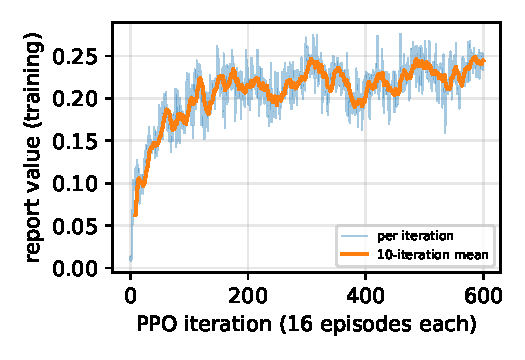
\includegraphics[width=\columnwidth]{figures/mappo_curve.pdf}
\caption{Training curve of the MAPPO baseline (B5): time-discounted report value per PPO iteration
and its 10-iteration mean. The return plateaus after about 150 iterations.}
\label{fig:mappo}
\end{figure}

\subsection{Onboard perception}\label{sec:eval:perception}
Table~\ref{tab:perception} compares YOLO26n with YOLOv8n trained under an identical protocol on
HIT-UAV \cite{hituav}. The two detectors reach the same mAP50 (0.948 vs.\ 0.947); YOLO26n is more
precise (0.932 vs.\ 0.909) and better localised (mAP50-95 0.533 vs.\ 0.520) with slightly lower
recall, and it needs 19\,\% fewer parameters and 31\,\% fewer operations. On a desktop GPU the two
are equally fast (about 1.8\,ms end-to-end with TensorRT FP16); we therefore attribute YOLO26n's
suitability for low-power hardware to its lower compute, not to measured speed, and we do not report
embedded latency, which was not measured. The accuracy values are the validation metrics recorded by
the training runs.
% generated by make_results.py -- do not edit by hand
\begin{table*}[t]\centering\caption{Thermal detectors trained with the same protocol (HIT-UAV, 100 epochs, AdamW, 640 px, seed 0). Accuracy: validation metrics recorded by the training run. Latency: end-to-end p50 on an RTX 3060 (desktop), PyTorch FP32 and TensorRT FP16.}\label{tab:perception}
\begin{tabular}{lcccccccc}\toprule
Model & Params [M] & GFLOPs & mAP50 & mAP50-95 & P & R & PyTorch [ms] & TensorRT [ms] \\\midrule
YOLO26n & 2.53 & 6.0 & 0.948 & 0.533 & 0.932 & 0.900 & 3.72 & 1.81 \\
YOLOv8n & 3.14 & 8.7 & 0.947 & 0.520 & 0.909 & 0.913 & 3.32 & 1.73 \\
\bottomrule\end{tabular}
\end{table*}


\subsection{Communication conditions}\label{sec:eval:channel}
Table~\ref{tab:e2} varies the channel from open terrain to the severe profile. SENTINEL reports the
largest share of victims within 60\,s in every profile and is significantly better than all seven
baselines in the open, suburban and urban settings (e.g.\ 0.575 vs.\ 0.475 for the best baseline,
B3, in urban rubble). In the severe channel it remains ahead (0.433 vs.\ 0.377) but the difference to
the best baseline is not significant. Its total share of reported victims is 0.56--0.58 across
profiles against 0.46--0.50 for the best baseline of each profile. In the severe profile SENTINEL's 90th-percentile
latency (99\,s) is longer than B0's (69\,s): it delivers more of the reports that would otherwise
never arrive, and some of these arrive late.
% generated by make_results.py -- do not edit by hand
\begin{table}[t]\centering\caption{Victims reported within 60 s per channel profile (N=8, 400 m, Poisson failures). Mean over 30 seeds; best per column in bold; $^*$: differs from SENTINEL (paired Wilcoxon, Holm-corrected, $p<0.05$).}\label{tab:e2}
\setlength{\tabcolsep}{4pt}\begin{adjustbox}{max width=\columnwidth}\begin{tabular}{lcccc}\toprule
Method & open & severe & suburban & urban \\\midrule
SENTINEL & \textbf{0.577} & \textbf{0.433} & \textbf{0.560} & \textbf{0.575} \\
B0 PSO & 0.473$^*$ & 0.377 & 0.456$^*$ & 0.453$^*$ \\
B1 Earlier design & 0.457$^*$ & 0.373 & 0.427$^*$ & 0.409$^*$ \\
B2 Comm-PSO & 0.472$^*$ & 0.336$^*$ & 0.371$^*$ & 0.468$^*$ \\
B3 $\lambda_2$-grad. & 0.477$^*$ & 0.353 & 0.453$^*$ & 0.475$^*$ \\
B4 Potential & 0.501$^*$ & 0.300$^*$ & 0.099$^*$ & 0.127$^*$ \\
B5 MAPPO & 0.405$^*$ & 0.333$^*$ & 0.421$^*$ & 0.396$^*$ \\
B6 Lawnmower & 0.424$^*$ & 0.373 & 0.423$^*$ & 0.421$^*$ \\
\bottomrule\end{tabular}\end{adjustbox}
\end{table}


\subsection{Failures}\label{sec:eval:failures}
Tables~\ref{tab:e3_urban_rubble} and~\ref{tab:e3_severe} apply six failure models: none, a single
crash, 30\,\% of the swarm crashing simultaneously, three cascading crashes, Poisson crashes at twice
the default rate, and a gradual transmit-power brownout. In the urban channel SENTINEL is
significantly better than every baseline under every failure model, by 23--30\,\% over the best
baseline. In the severe channel it is ahead of or tied with the best baseline (often the lawnmower
sweep), with no significant loss. Information loss, i.e.\ confirmed victims whose every holder
failed before reporting, is small for \emph{all} methods: at most 0.9\,\% averaged over all failure
models and at most 8.5\,\% under high-rate Poisson crashes in the severe channel (3.2\,\% for
SENTINEL). Gossip replication between UAVs that meet during the search protects most information,
so we make no claim that SENTINEL reduces loss compared with the baselines.
% generated by make_results.py -- do not edit by hand
\begin{table*}[t]\centering\caption{Victims reported within 60 s under failure models (urban-rubble channel, N=8, 400 m). Mean over 30 seeds; best per column in bold; $^*$: differs from SENTINEL (paired Wilcoxon, Holm-corrected, $p<0.05$).}\label{tab:e3_urban_rubble}
\setlength{\tabcolsep}{4pt}\begin{adjustbox}{max width=\textwidth}\begin{tabular}{lcccccc}\toprule
Method & brownout & cascading & none & Poisson & 30\\% simult. & single \\\midrule
SENTINEL & \textbf{0.687} & \textbf{0.643} & \textbf{0.691} & \textbf{0.459} & \textbf{0.675} & \textbf{0.689} \\
B0 PSO & 0.539$^*$ & 0.509$^*$ & 0.537$^*$ & 0.344$^*$ & 0.513$^*$ & 0.523$^*$ \\
B1 Earlier design & 0.513$^*$ & 0.495$^*$ & 0.501$^*$ & 0.356$^*$ & 0.499$^*$ & 0.501$^*$ \\
B2 Comm-PSO & 0.555$^*$ & 0.524$^*$ & 0.560$^*$ & 0.340$^*$ & 0.521$^*$ & 0.545$^*$ \\
B3 $\lambda_2$-grad. & 0.532$^*$ & 0.489$^*$ & 0.533$^*$ & 0.339$^*$ & 0.505$^*$ & 0.523$^*$ \\
B4 Potential & 0.183$^*$ & 0.161$^*$ & 0.193$^*$ & 0.085$^*$ & 0.144$^*$ & 0.160$^*$ \\
B5 MAPPO & 0.489$^*$ & 0.457$^*$ & 0.499$^*$ & 0.328$^*$ & 0.453$^*$ & 0.473$^*$ \\
B6 Lawnmower & 0.521$^*$ & 0.488$^*$ & 0.521$^*$ & 0.345$^*$ & 0.485$^*$ & 0.511$^*$ \\
\bottomrule\end{tabular}\end{adjustbox}
\end{table*}

% generated by make_results.py -- do not edit by hand
\begin{table*}[t]\centering\caption{Victims reported within 60 s under failure models (severe channel, N=8, 400 m). Mean over 30 seeds; best per column in bold; $^*$: differs from SENTINEL (paired Wilcoxon, Holm-corrected, $p<0.05$).}\label{tab:e3_severe}
\setlength{\tabcolsep}{4pt}\begin{adjustbox}{max width=\textwidth}\begin{tabular}{lcccccc}\toprule
Method & brownout & cascading & none & Poisson & 30\\% simult. & single \\\midrule
SENTINEL & \textbf{0.517} & 0.452 & \textbf{0.529} & \textbf{0.340} & \textbf{0.496} & \textbf{0.512} \\
B0 PSO & 0.444 & 0.403 & 0.456 & 0.291 & 0.417 & 0.440 \\
B1 Earlier design & 0.448 & 0.423 & 0.469 & 0.295 & 0.440 & 0.452 \\
B2 Comm-PSO & 0.427$^*$ & 0.385 & 0.439$^*$ & 0.259$^*$ & 0.400$^*$ & 0.428 \\
B3 $\lambda_2$-grad. & 0.380$^*$ & 0.363$^*$ & 0.409$^*$ & 0.249$^*$ & 0.392$^*$ & 0.409$^*$ \\
B4 Potential & 0.359$^*$ & 0.309$^*$ & 0.396$^*$ & 0.200$^*$ & 0.359$^*$ & 0.361$^*$ \\
B5 MAPPO & 0.431$^*$ & 0.383 & 0.445$^*$ & 0.267$^*$ & 0.412$^*$ & 0.440$^*$ \\
B6 Lawnmower & 0.499 & \textbf{0.453} & 0.508 & 0.287 & 0.468 & 0.495 \\
\bottomrule\end{tabular}\end{adjustbox}
\end{table*}


\subsection{Scalability}\label{sec:eval:scal}
Tables~\ref{tab:e1_400} and~\ref{tab:e1_200} vary the swarm from 3 to 50 UAVs. On the 400\,m area
SENTINEL is significantly better than all baselines at every swarm size, from 0.203 vs.\ 0.153 with
three UAVs to 0.788 vs.\ 0.725 with fifty. On the smaller 200\,m area, where contacts are frequent,
it has the highest mean at every swarm size but is significantly better than all baselines only for
$N=50$ (0.809 vs.\ 0.779). In dense swarms MAPPO (B5) becomes the strongest baseline (0.691--0.779
for $N\ge10$ on the 200\,m area), while it remains well behind in sparse settings. The per-agent planning time
grows with the number of neighbours a UAV hears, not with $N$ directly: from 4.0 to 11.1\,ms on the
dense 200\,m area and from 5.1 to 9.5\,ms on the 400\,m area as $N$ grows from 3 to 50
(Fig.~\ref{fig:compute}), far below the 1\,s planning period. The all-neighbour communication-aware
PSO (B2) grows faster, to 20.6\,ms.
% generated by make_results.py -- do not edit by hand
\begin{table}[t]\centering\caption{Victims reported within 60 s vs swarm size N (400 m map, urban, Poisson failures). Mean over 30 seeds; best per column in bold; $^*$: differs from SENTINEL (paired Wilcoxon, Holm-corrected, $p<0.05$).}\label{tab:e1_400}
\setlength{\tabcolsep}{4pt}\begin{adjustbox}{max width=\columnwidth}\begin{tabular}{lccccc}\toprule
Method & N=3 & N=5 & N=10 & N=20 & N=50 \\\midrule
SENTINEL & \textbf{0.203} & \textbf{0.389} & \textbf{0.667} & \textbf{0.751} & \textbf{0.788} \\
B0 PSO & 0.153$^*$ & 0.285$^*$ & 0.535$^*$ & 0.619$^*$ & 0.656$^*$ \\
B1 Earlier design & 0.109$^*$ & 0.232$^*$ & 0.499$^*$ & 0.647$^*$ & 0.707$^*$ \\
B2 Comm-PSO & 0.147$^*$ & 0.313$^*$ & 0.535$^*$ & 0.641$^*$ & 0.685$^*$ \\
B3 $\lambda_2$-grad. & 0.136$^*$ & 0.273$^*$ & 0.529$^*$ & 0.636$^*$ & 0.665$^*$ \\
B4 Potential & 0.017$^*$ & 0.027$^*$ & 0.240$^*$ & 0.485$^*$ & 0.712$^*$ \\
B5 MAPPO & 0.153$^*$ & 0.273$^*$ & 0.503$^*$ & 0.628$^*$ & 0.725$^*$ \\
B6 Lawnmower & 0.151$^*$ & 0.265$^*$ & 0.444$^*$ & 0.493$^*$ & 0.619$^*$ \\
\bottomrule\end{tabular}\end{adjustbox}
\end{table}

% generated by make_results.py -- do not edit by hand
\begin{table}[t]\centering\caption{Victims reported within 60 s vs swarm size N (200 m map, urban, Poisson failures). Mean over 30 seeds; best per column in bold; $^*$: differs from SENTINEL (paired Wilcoxon, Holm-corrected, $p<0.05$).}\label{tab:e1_200}
\setlength{\tabcolsep}{4pt}\begin{adjustbox}{max width=\columnwidth}\begin{tabular}{lccccc}\toprule
Method & N=3 & N=5 & N=10 & N=20 & N=50 \\\midrule
SENTINEL & \textbf{0.475} & \textbf{0.620} & \textbf{0.720} & \textbf{0.743} & \textbf{0.809} \\
B0 PSO & 0.457 & 0.597 & 0.660$^*$ & 0.697$^*$ & 0.720$^*$ \\
B1 Earlier design & 0.360$^*$ & 0.565 & 0.652$^*$ & 0.692$^*$ & 0.724$^*$ \\
B2 Comm-PSO & 0.459 & 0.579 & 0.647$^*$ & 0.725 & 0.732$^*$ \\
B3 $\lambda_2$-grad. & 0.345$^*$ & 0.560 & 0.664$^*$ & 0.695$^*$ & 0.727$^*$ \\
B4 Potential & 0.044$^*$ & 0.112$^*$ & 0.471$^*$ & 0.656$^*$ & 0.735$^*$ \\
B5 MAPPO & 0.379 & 0.559 & 0.691 & 0.729 & 0.779$^*$ \\
B6 Lawnmower & 0.419 & 0.536$^*$ & 0.541$^*$ & 0.641$^*$ & 0.703$^*$ \\
\bottomrule\end{tabular}\end{adjustbox}
\end{table}

\begin{figure}[t]\centering
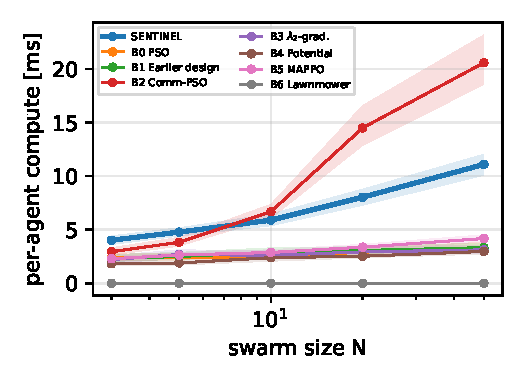
\includegraphics[width=\columnwidth]{figures/e1_compute_200m.pdf}
\caption{Per-agent planning time vs.\ swarm size on the 200\,m area (mean and 95\,\% CI over 30 seeds).}
\label{fig:compute}
\end{figure}

\subsection{Moving obstacles}\label{sec:eval:dynamic}
With 5 or 15 tall debris objects drifting through the area, blocking links and hiding victims
(Table~\ref{tab:e4}), SENTINEL keeps reporting 0.58 of the victims within 60\,s and remains
significantly better than all baselines (best baseline 0.48--0.51).
% generated by make_results.py -- do not edit by hand
\begin{table}[t]\centering\caption{Victims reported within 60 s with moving obstacles (urban, N=8). Mean over 30 seeds; best per column in bold; $^*$: differs from SENTINEL (paired Wilcoxon, Holm-corrected, $p<0.05$).}\label{tab:e4}
\setlength{\tabcolsep}{4pt}\begin{adjustbox}{max width=\columnwidth}\begin{tabular}{lccc}\toprule
Method & 0 moving & 5 moving & 15 moving \\\midrule
SENTINEL & \textbf{0.575} & \textbf{0.585} & \textbf{0.579} \\
B0 PSO & 0.453$^*$ & 0.481$^*$ & 0.460$^*$ \\
B1 Earlier design & 0.409$^*$ & 0.424$^*$ & 0.447$^*$ \\
B2 Comm-PSO & 0.468$^*$ & 0.489$^*$ & 0.509$^*$ \\
B3 $\lambda_2$-grad. & 0.475$^*$ & 0.479$^*$ & 0.487$^*$ \\
B4 Potential & 0.127$^*$ & 0.132$^*$ & 0.141$^*$ \\
B5 MAPPO & 0.396$^*$ & 0.449$^*$ & 0.431$^*$ \\
B6 Lawnmower & 0.421$^*$ & 0.443$^*$ & 0.425$^*$ \\
\bottomrule\end{tabular}\end{adjustbox}
\end{table}


\subsection{Detection uncertainty}\label{sec:eval:uncertainty}
We perturbed the calibrated detector model around its default: confidence noise
$\sigma\in\{0.04,0.08,0.15,0.25\}$, a weaker detector ($c_{\max}\in\{0.8,0.7\}$) and more frequent
false alarms. SENTINEL stays significantly ahead of B0 and B6 in all eight settings (0.45--0.81 vs.\
at most 0.59). Because the default false-alarm confidences rarely exceed the confirmation threshold,
we also ran a deliberately adverse case (Table~\ref{tab:e6c}): hot clutter that scores up to a mean of
0.55, the confidence noise applied to false alarms as well, and false alarms three times more
frequent. SENTINEL still reports 0.71--0.73 of the victims within 60\,s against at most 0.50 (B0), with
0.18 false confirmed entries per mission on average (B0: 0.29). Moving the SA band and the
confirmation threshold (0.3/0.6 to 0.4/0.85) changes the on-time share between 0.64 and 0.74 without
producing false confirmations.
% generated by make_results.py -- do not edit by hand
\begin{table}[t]\centering\caption{Victims reported within 60 s with hot-clutter false alarms (urban, N=8, $\sigma$=0.15). Mean over 30 seeds; best per column in bold; $^*$: differs from SENTINEL (paired Wilcoxon, Holm-corrected, $p<0.05$).}\label{tab:e6c}
\setlength{\tabcolsep}{4pt}\begin{adjustbox}{max width=\columnwidth}\begin{tabular}{lcccc}\toprule
Method & $\mu_{\mathrm{fp}}$=0.22, $r$=0.1 & $\mu_{\mathrm{fp}}$=0.4, $r$=0.1 & $\mu_{\mathrm{fp}}$=0.55, $r$=0.1 & $\mu_{\mathrm{fp}}$=0.55, $r$=0.3 \\\midrule
SENTINEL & \textbf{0.731} & \textbf{0.719} & \textbf{0.724} & \textbf{0.709} \\
B0 PSO & 0.501$^*$ & 0.491$^*$ & 0.500$^*$ & 0.493$^*$ \\
B6 Lawnmower & 0.480$^*$ & 0.480$^*$ & 0.479$^*$ & 0.481$^*$ \\
no SA & 0.715 & 0.693 & 0.708 & 0.668 \\
no fusion & 0.672$^*$ & 0.655$^*$ & 0.676$^*$ & 0.691 \\
\bottomrule\end{tabular}\end{adjustbox}
\end{table}


\subsection{What produces the gains}\label{sec:eval:ablation}
Table~\ref{tab:e7} removes one component at a time. Two components matter. First, multi-view fusion:
removing it reduces on-time reports significantly (urban, $N=8$: 0.519 vs.\ 0.575), and in the dense
swarm of Table~\ref{tab:e11_dense_diag} the corroborative rule is decisive (0.809, against 0.656 with
plain naive-Bayes fusion and 0.720 for B0). Second, the delivery trigger: Fig.~\ref{fig:thold} sweeps
$T_h$; in the severe channel with eight UAVs, delivering immediately ($T_h=0$) raises the on-time
share from 0.388 (never delivering) to 0.497 and lowers the 90th-percentile latency from 97\,s to
34\,s, while the total share of reported victims stays at 0.50. In the urban channel the same trend is
present but not significant. The remaining components (outage-based instead of distance-based spring,
LMST instead of nearest-neighbour preserved set, information-dependent tension, projection) do not
change the outcome significantly, and the SA flank is not significant in the tuned configuration.
These mechanisms act only during the short delivery tethers; we regard them as the safety layer
examined next, not as the source of the performance gains. Keeping the swarm connected at all times
(SENTINEL-strict) lowers on-time reporting to 0.03--0.13.
% generated by make_results.py -- do not edit by hand
\begin{table}[t]\centering\caption{Ablation: victims reported within 60 s (400 m, Poisson failures). Mean over 30 seeds; best per column in bold; $^*$: differs from SENTINEL (paired Wilcoxon, Holm-corrected, $p<0.05$).}\label{tab:e7}
\setlength{\tabcolsep}{4pt}\begin{adjustbox}{max width=\columnwidth}\begin{tabular}{lcccc}\toprule
Method & severe, N=4 & severe, N=8 & urban, N=4 & urban, N=8 \\\midrule
SENTINEL & \textbf{0.212} & 0.433 & 0.313 & 0.575 \\
SENTINEL-strict & 0.029$^*$ & 0.061$^*$ & 0.064$^*$ & 0.131$^*$ \\
distance spring & 0.200 & 0.433 & 0.307 & 0.561 \\
NN set & \textbf{0.212} & 0.433 & 0.313 & 0.573 \\
no info. tension & 0.211 & 0.433 & 0.312 & 0.572 \\
no projection & 0.200 & 0.435 & 0.308 & 0.545 \\
no SA & 0.189 & \textbf{0.455} & \textbf{0.316} & \textbf{0.583} \\
no fusion & 0.187 & 0.408 & 0.288 & 0.519$^*$ \\
naive-Bayes fusion & 0.167 & 0.439 & 0.300 & 0.540 \\
\bottomrule\end{tabular}\end{adjustbox}
\end{table}

% generated by make_results.py -- do not edit by hand
\begin{table}[t]\centering\caption{Dense swarm (200 m, N=50): victims reported within 60 s; ablations of SENTINEL and baselines with its fusion rule (same seeds). Mean over 30 seeds; best in bold; $^*$: differs from SENTINEL (paired Wilcoxon, Holm-corrected, $p<0.05$).}\label{tab:e11_dense_diag}
\setlength{\tabcolsep}{4pt}\begin{adjustbox}{max width=\columnwidth}\begin{tabular}{lc}\toprule
Method & 50 \\\midrule
SENTINEL & 0.809 \\
B0 PSO & 0.720$^*$ \\
no SA & 0.799 \\
no fusion & 0.740$^*$ \\
naive-Bayes fusion & 0.656$^*$ \\
no SA, no fusion & 0.719$^*$ \\
B0 + fusion & 0.815 \\
B1 + fusion & 0.819 \\
B2 + fusion & 0.833 \\
B3 + fusion & 0.815 \\
B4 + fusion & \textbf{0.865$^*$} \\
B5 + fusion & 0.819 \\
B6 + fusion & 0.849 \\
\bottomrule\end{tabular}\end{adjustbox}
\end{table}

\begin{figure}[t]\centering
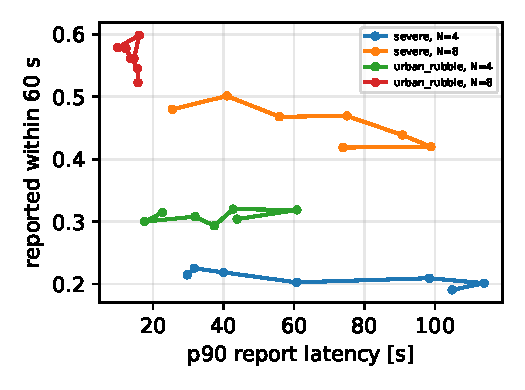
\includegraphics[width=\columnwidth]{figures/e10_thold_tradeoff.pdf}
\caption{Delivery trigger $T_h\in\{0,15,30,60,120,240,\infty\}$: on-time share vs.\ 90th-percentile
report latency for four regimes (each point: mean of 30 seeds).}
\label{fig:thold}
\end{figure}

\subsection{Link preservation during delivery}\label{sec:eval:safety}
Proposition~\ref{prop:link} is a one-step guarantee for feasible steps. Over all experiments we
counted the tethered, mutually preserved links that were reliable before a step and unreliable after
it: 15 violations in 436\,057 link-steps ($3.4\times10^{-5}$); with the swarm tethered at all times
(SENTINEL-strict) the rate is $2.6\times10^{-3}$. The residual violations come from steps where the
constraint was infeasible and the UAV hovered (Section~\ref{sec:proj}). Information loss did not vary
consistently with $T_h$ at the failure rates studied (at most 6.2\,\% in any cell), so the exposure
bound of Proposition~\ref{prop:exposure} could not be confirmed or refuted empirically; it remains a
design guarantee.

\subsection{Cross-validation in PX4/Gazebo and the earlier scenario}\label{sec:eval:sitl}
To check that the fast simulator does not depend on idealised flight, we flew SENTINEL and B0 with
three PX4 x500 multicopters in Gazebo Harmonic on the same three 100\,m areas and seeds (300\,s,
crash of one UAV at 150\,s), with the same agent code, tuned values, channel emulation and detector
model. The share of reported victims (SENTINEL 0.53 vs.\ 0.60 in the fast simulator; B0 0.60 vs.\
0.62), the packet delivery ratio (0.79--0.81 vs.\ 0.80--0.83) and the connected fraction agree within
0.07; coverage of SENTINEL is higher in SITL (0.99 vs.\ 0.83). With three seeds this is a consistency
check rather than a statistical comparison. Finally, re-running the scenario of the earlier SENTINEL design
(25\,m area, three UAVs, one crash) shows that it cannot separate the methods: the
area is far smaller than the radio range, every method stays connected throughout, and 64--69\,\% of
the victims are reported by all of them. The remaining victims are either buried or so close to
another victim (4--5\,m) that their reports merge (7.8--11\,\% of confirmations), which is a
limitation of the association gate rather than of connectivity.

\section{Discussion and Limitations}\label{sec:discussion}

\paragraph{Where the gains come from}
The experiments support a narrower claim than "keeping the network alive". Connectivity in itself
is not the bottleneck in the scenarios we studied: keeping the swarm connected at all times
(SENTINEL-strict, B3, B4) limits the search and lowers on-time reporting, and gossip between UAVs
that meet during the search already protects most information from failures. What raised timely
reporting was deciding \emph{when} a UAV should stop searching to deliver what it found, and
combining views so that occlusion does not hide confirmed victims; these are the components with
significant effects. Given the same fusion rule, the baselines remain significantly behind in the
urban 400\,m scenarios, but in a dense 50-UAV swarm they match SENTINEL and one exceeds it, so there
the fusion rule, not the mobility, is what matters. Part
of its margin in the urban default is not explained by these components
(Section~\ref{sec:eval:ablation}). The link-preservation layer (Proposition~\ref{prop:link}) did not
change the on-time share measurably, but it reduced preserved-link violations 37-fold; its role is to
make deliveries reliable when they happen.

\paragraph{Choice of $T_h$}
$T_h$ trades on-time reporting against total discovery. The value tuned on the report value $J$
(116\,s) is longer than the 60\,s deadline. It still improves on-time reporting over never
delivering (urban, $N=8$: 0.577 at $T_h=120$\,s vs.\ 0.523), but a hold time of 15\,s was better in
both channels with eight UAVs (0.599 urban, 0.501 severe; Fig.~\ref{fig:thold}). In practice $T_h$ should follow the responders' reporting deadline; adapting it online to the
observed contact rate is a natural extension.

\paragraph{Tuning sensitivity}
An earlier configuration of SENTINEL that also tethered UAVs softly while exploring helped dense
swarms but reduced coverage in the severe channel; the evaluated design does not use this tether.
Results of that configuration are released with the others.

\paragraph{Limitations}
(i)~All results are from simulation: a fast multi-agent simulator and PX4 software-in-the-loop in
Gazebo; no hardware flights were performed. (ii)~The channel model is parameterised from published
ranges and has not been calibrated against measurements in rubble. (iii)~Detection accuracy is
reported from the validation split recorded by the training runs; the detector transfers poorly to
rendered thermal scenes, which is why the in-the-loop comparison uses the detector model; that
model's parameters were chosen to reproduce the detector's qualitative behaviour and swept, not
fitted to detector outputs.
(iv)~Victims closer than the association gate (about 5\,m) can be merged into one report.
(v)~MAPPO was trained to a plateau (600 iterations) with one observation and reward design; other
MARL formulations may perform better, in particular in dense swarms, where it is already the strongest
baseline. (vi)~The exposure bound
(Proposition~\ref{prop:exposure}) could not be tested empirically because losses were rare at the
failure rates studied. (vii)~Latency was measured on a desktop GPU, not on embedded hardware.

\section{Conclusion}\label{sec:conclusion}

We studied how a UAV swarm without infrastructure can get victim reports to responders in time.
SENTINEL lets UAVs search freely, triggers delivery from the information each UAV has confirmed,
fuses views so that occluded angles cannot veto a clear detection, and preserves the links of a
delivery path for every feasible step (Proposition~\ref{prop:link}). In about 13\,000 simulated missions against seven
tuned baselines, it reported significantly more victims within 60\,s than every baseline in most
settings (urban, suburban and open channels, all failure settings in urban rubble, swarms of 3--50
UAVs on the 400\,m area and moving obstacles), it stayed significantly ahead of the two baselines
tested under detector uncertainty, in the severe channel it was ahead of or tied with the best
baseline, and it was never significantly worse than any of the seven baselines. A PX4/Gazebo cross-check
agreed with the fast simulator within 0.07.
The ablation found significant effects for the fusion rule and the delivery trigger; in the urban
400\,m scenarios SENTINEL remained significantly ahead when the baselines were given its fusion rule,
whereas in a dense 50-UAV swarm the fusion rule alone explained its advantage. Continuous connectivity
did not help, and the link-preservation layer reduced preserved-link violations 37-fold. Future work will adapt the delivery trigger to the observed contact rate,
calibrate the channel model with measurements, and validate the system in hardware flights.


\bibliographystyle{IEEEtran}
\bibliography{references}
\end{document}
